\chapter{Design and test specification} \label{ch:req}
This chapter contains the requirements for the system and a test specification which will describe how to test for the requirements.\\

A way to identify the performance of a design using different design metrics is the cost function. The cost function is the overall cost of a design and is a function of the different design metric:
\begin{equation}
C = f(A,T,P,N,test) = a_1\cdot A + a_2 \cdot T + a_3 \cdot P + a_4 \cdot N + a_4 \cdot test
\end{equation}
where $A$ is area, $T$ is time, $P$ is power, $N$ is noise, $test$ is the result from middlebury test and $a_i$ tells the importance of the associated metric.\\
It is the task of the system designer to minimize this cost. And due to $a_i$ the cost function can be changed to fit the priorities of the application.\\

For this thesis the number one priority is the time metric since it is wished for the algorithm to be real-time. The test metric is also important since it describes the quality of the stereo matching. Area isn't as important because if the target FPGA is to small then HSA systems will use a larger FPGA but larger area often equals more expensive hardware. Power isn't important either since the stereo setup is intended being a part of industrial systems hence power is easily accessible.\\
An ordered list of priorities for the design metrics in this project:
\begin{enumerate}
  \item Time
  \item Test
  \item Area
  \item Power
  \item Noise
\end{enumerate}

In this thesis the cost function will be used when choosing e.g when comparing the different algorithms found in chapter \vref{ch:algdesign}. 

\section{Requirement specification}
\begin{table}[ht!]
  \centering
  \begin{tabular}{l l c c p{4cm} p{2.5cm}}
  \toprule
  \textbf{No.} & \textbf{Parameter} & \textbf{Value} & \textbf{Unit} & \textbf{Additional Information} & \textbf{Source} \\
  \midrule
  1 & Frame rate & $\geq 10$ & fps & & Section \vref{sec:intromotiv} \\
  \midrule
  2 & Disparity precision & $\leq 2$ & mm & $\bullet$ Either directly or using subpixel refinement \newline $\bullet$ In the range 0.5-\SI{1.5}{\meter} & Section \vref{sec:intromotiv}\\
  \midrule
  3 & Camera resolution & 2592$\times$1944 & pixels & & Section \vref{sec:disppre} \\
  \midrule
  4 & Focal length & $\geq 10$ & mm & & Section \vref{sec:disppre} \\
  \midrule
  5 & Pixel size & 0.0022 & \si{\micro\meter} & & Section \vref{sec:disppre} \\  
  \bottomrule
  \end{tabular}
\end{table}
\section{Test specification}
This section will describe how to the requirements can be tested to ensure that they are fulfilled. \\

Requirement 1: frame rate can be tested by running the finalized implementation and measure the run time which then should be \SI{\leq 100}{\milli\second}. \\

Requirement 2: disparity precision. For this HSA systems has produced a test object which has small depth increases. Figure \vref{fig:3dpretest} shows a 3D model of this test object. This model was 3D printed in case a working prototype of the prototype was available for testing. The steps closest to the bottom right of the figure increase by 1 mm for each step. The next line increase by 2 mm for each step. This continues and the last line of steps increases by 5 mm for each step. The small shapes in the middle of each step have a depth difference of 0.5 mm and alternately protrudes from or recesses into the steps. This object can be used to test where the precision of a stereo setup and algorithm is between 0.5 and 5 mm depending on which lines of step can be seen. \\

\begin{figure}[ht!]
  \centering
  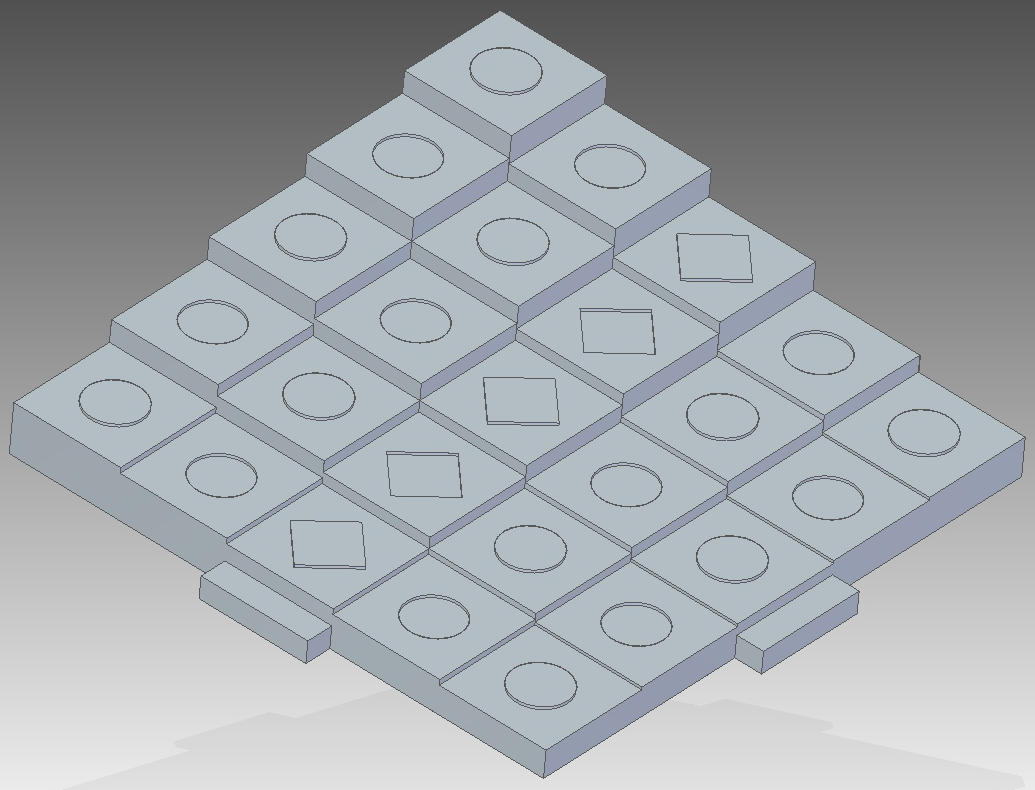
\includegraphics[width=0.5\textwidth]{figures/3dprecisiontest}
  \caption{3D model of test object for depth precision}
  \label{fig:3dpretest}
\end{figure}
The middlebury test set does not contain images where specific areas contain depth increments of 2 mm and therefore these images can not be used for testing this requirement and calculations \vref{sec:disppre} are used instead. \\


Requirement 3: camera resolution, requirement 4: focal length and requirement 5: pixel size are fulfilled by choosing the correct camera hardware but are essential to be fulfilled for requirement 2 to be fulfilled.\\

Chapter \vref{ch:acctest} will perform the available tests.

